\section{Half-Edge Mesh}
Um ein Traversieren eines Meshes, Abfragen der Nachbarschaftsbeziehungen der einzelnen Meshkomponenten so und Operationen wie ,,Subdivisionen'' von Faces (Unterteilung der Faces in kleinere Dreiecke) einfach wie m\"oglich zu machen, gibt es neben den oben genannten Ans\"atzen noch den Ansatz der Half-Edge Meshes. Ein solches Mesh besteht aus folgenden Komponenten:
\begin{itemize}
	\item eine Liste von Vertices
	\item eine Liste von Half-Edges
	\item eine Liste von Faces.
\end{itemize}

\begin{figure}[h]
	\centering
	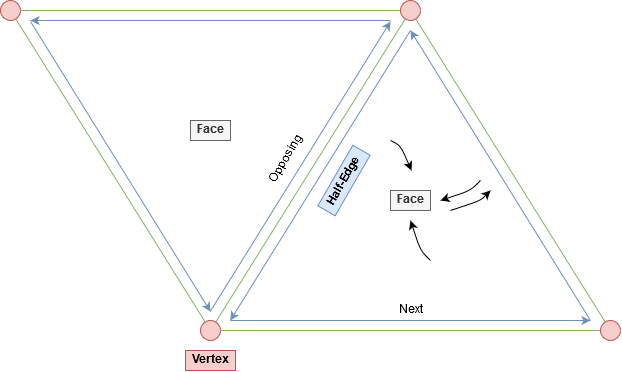
\includegraphics[width=0.7\linewidth]{Images/half-edge-mesh}
	\caption[Half-Edge-Mesh Schematik]{Die Elemente eines Half-Edge-Mesh.}
	\label{fig:half-edge-mesh}
\end{figure}

Im Gegensatz zu den Winged-Edge Meshes modellieren die Half-Edge Meshes eine Kante nicht explizit, sondern als Kombination aus zwei Half-Edges, die in jeweils entgegengesetzte Richtungen auf einen der Endpunkte der Kante zeigen. Durch die Aufteilung der Kanten kann jede Half-Edge genau einer Face zugeordnet werden und besitzt somit nicht mehr eine Referenz auf den linken und rechten Nachfolger, sondern einen nur noch einen Pointer auf die n\"achste Half-Edge der Face, wie in Abbildung \ref{fig:half-edge-mesh} gezeigt. Zudem Besitzt jede Half-Edge einen Verweis auf die zugeh\"orige Face sowie auf die Gegen\"uberliegende Half-Edge. Ein Verweis auf die Vorherige ist nicht n\"otig, da diese die \"ubern\"achste Kante ist. 

\subsection{Vergleich mir anderen Datenstrukturen}
\subsection{}